\section{研究背景}
%TODO:初号機体のお話を書く
当研究室において先行研究として、人間の筋肉を模した空気圧人工筋をもちいたペダリングロボット(初号機)が存在する.これは,人間のペダリング動作の計測を行い、ロボットに再現させるものであった。
\begin{figure}
 \begin{center}
  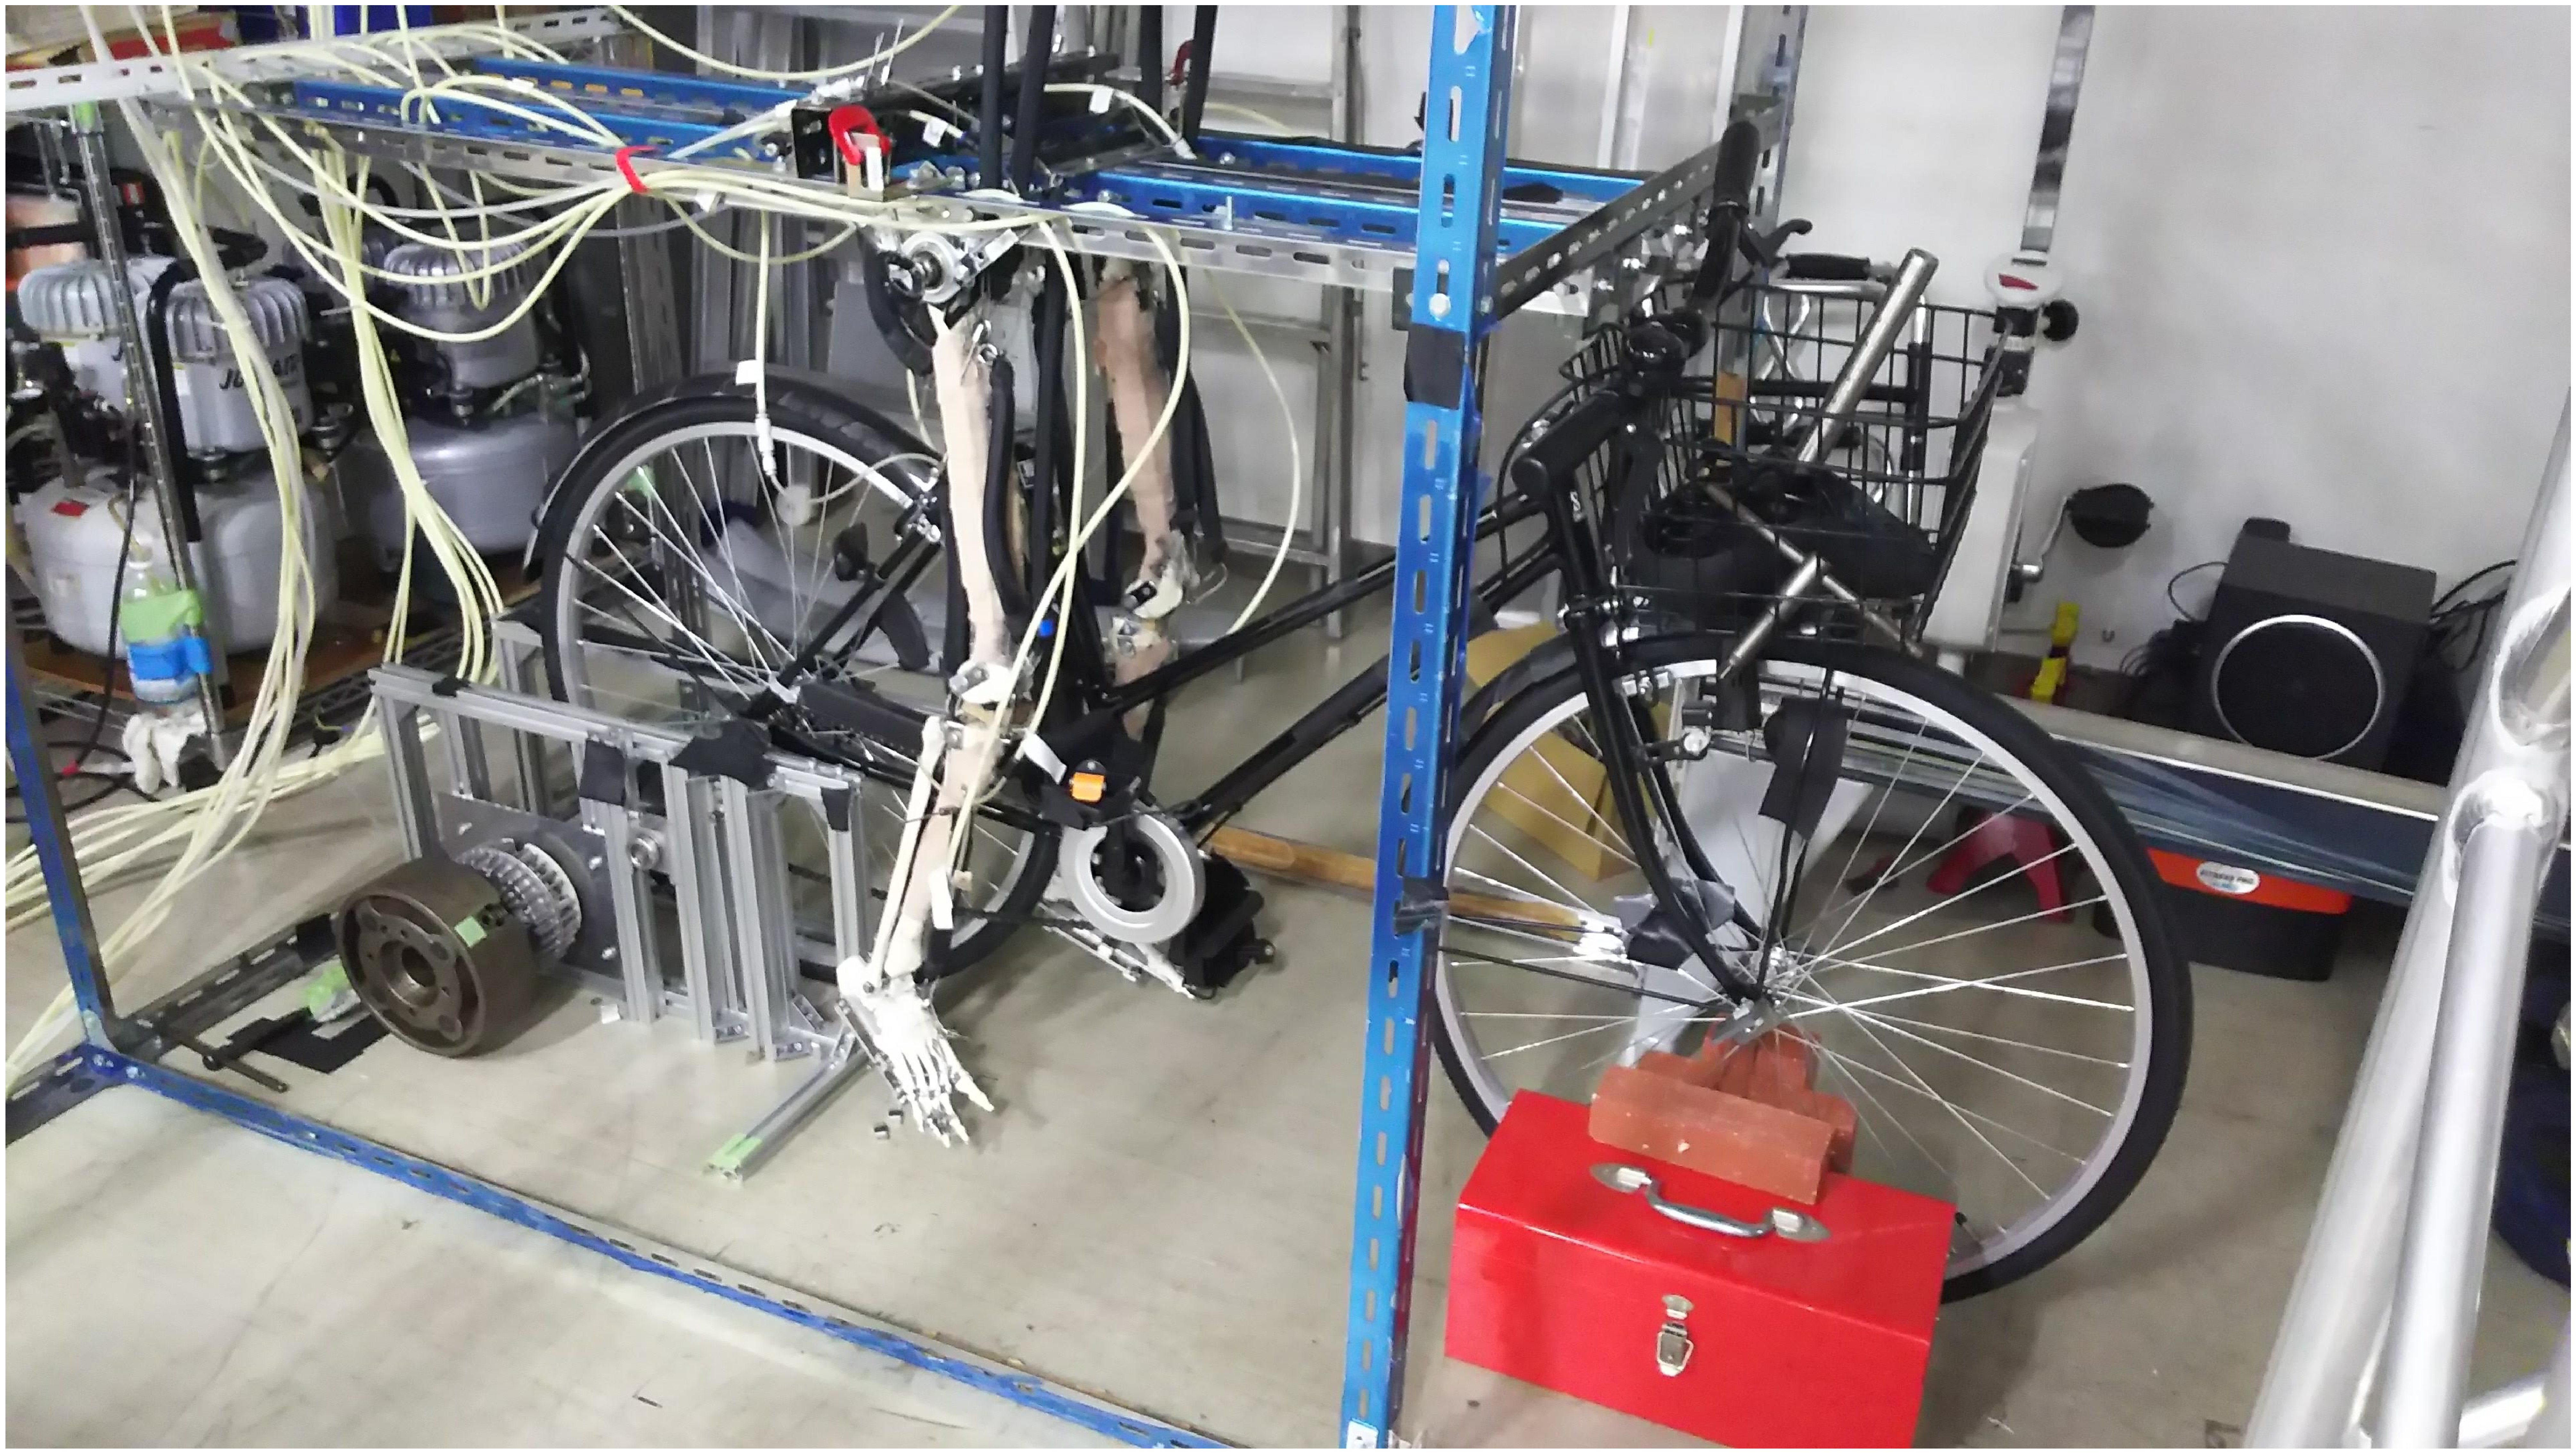
\includegraphics[width=0.5\columnwidth,clip]{Photo/BackGround/1st.eps}
  \caption{ペダリングロボット(初号機)}
  \label{初号機}
  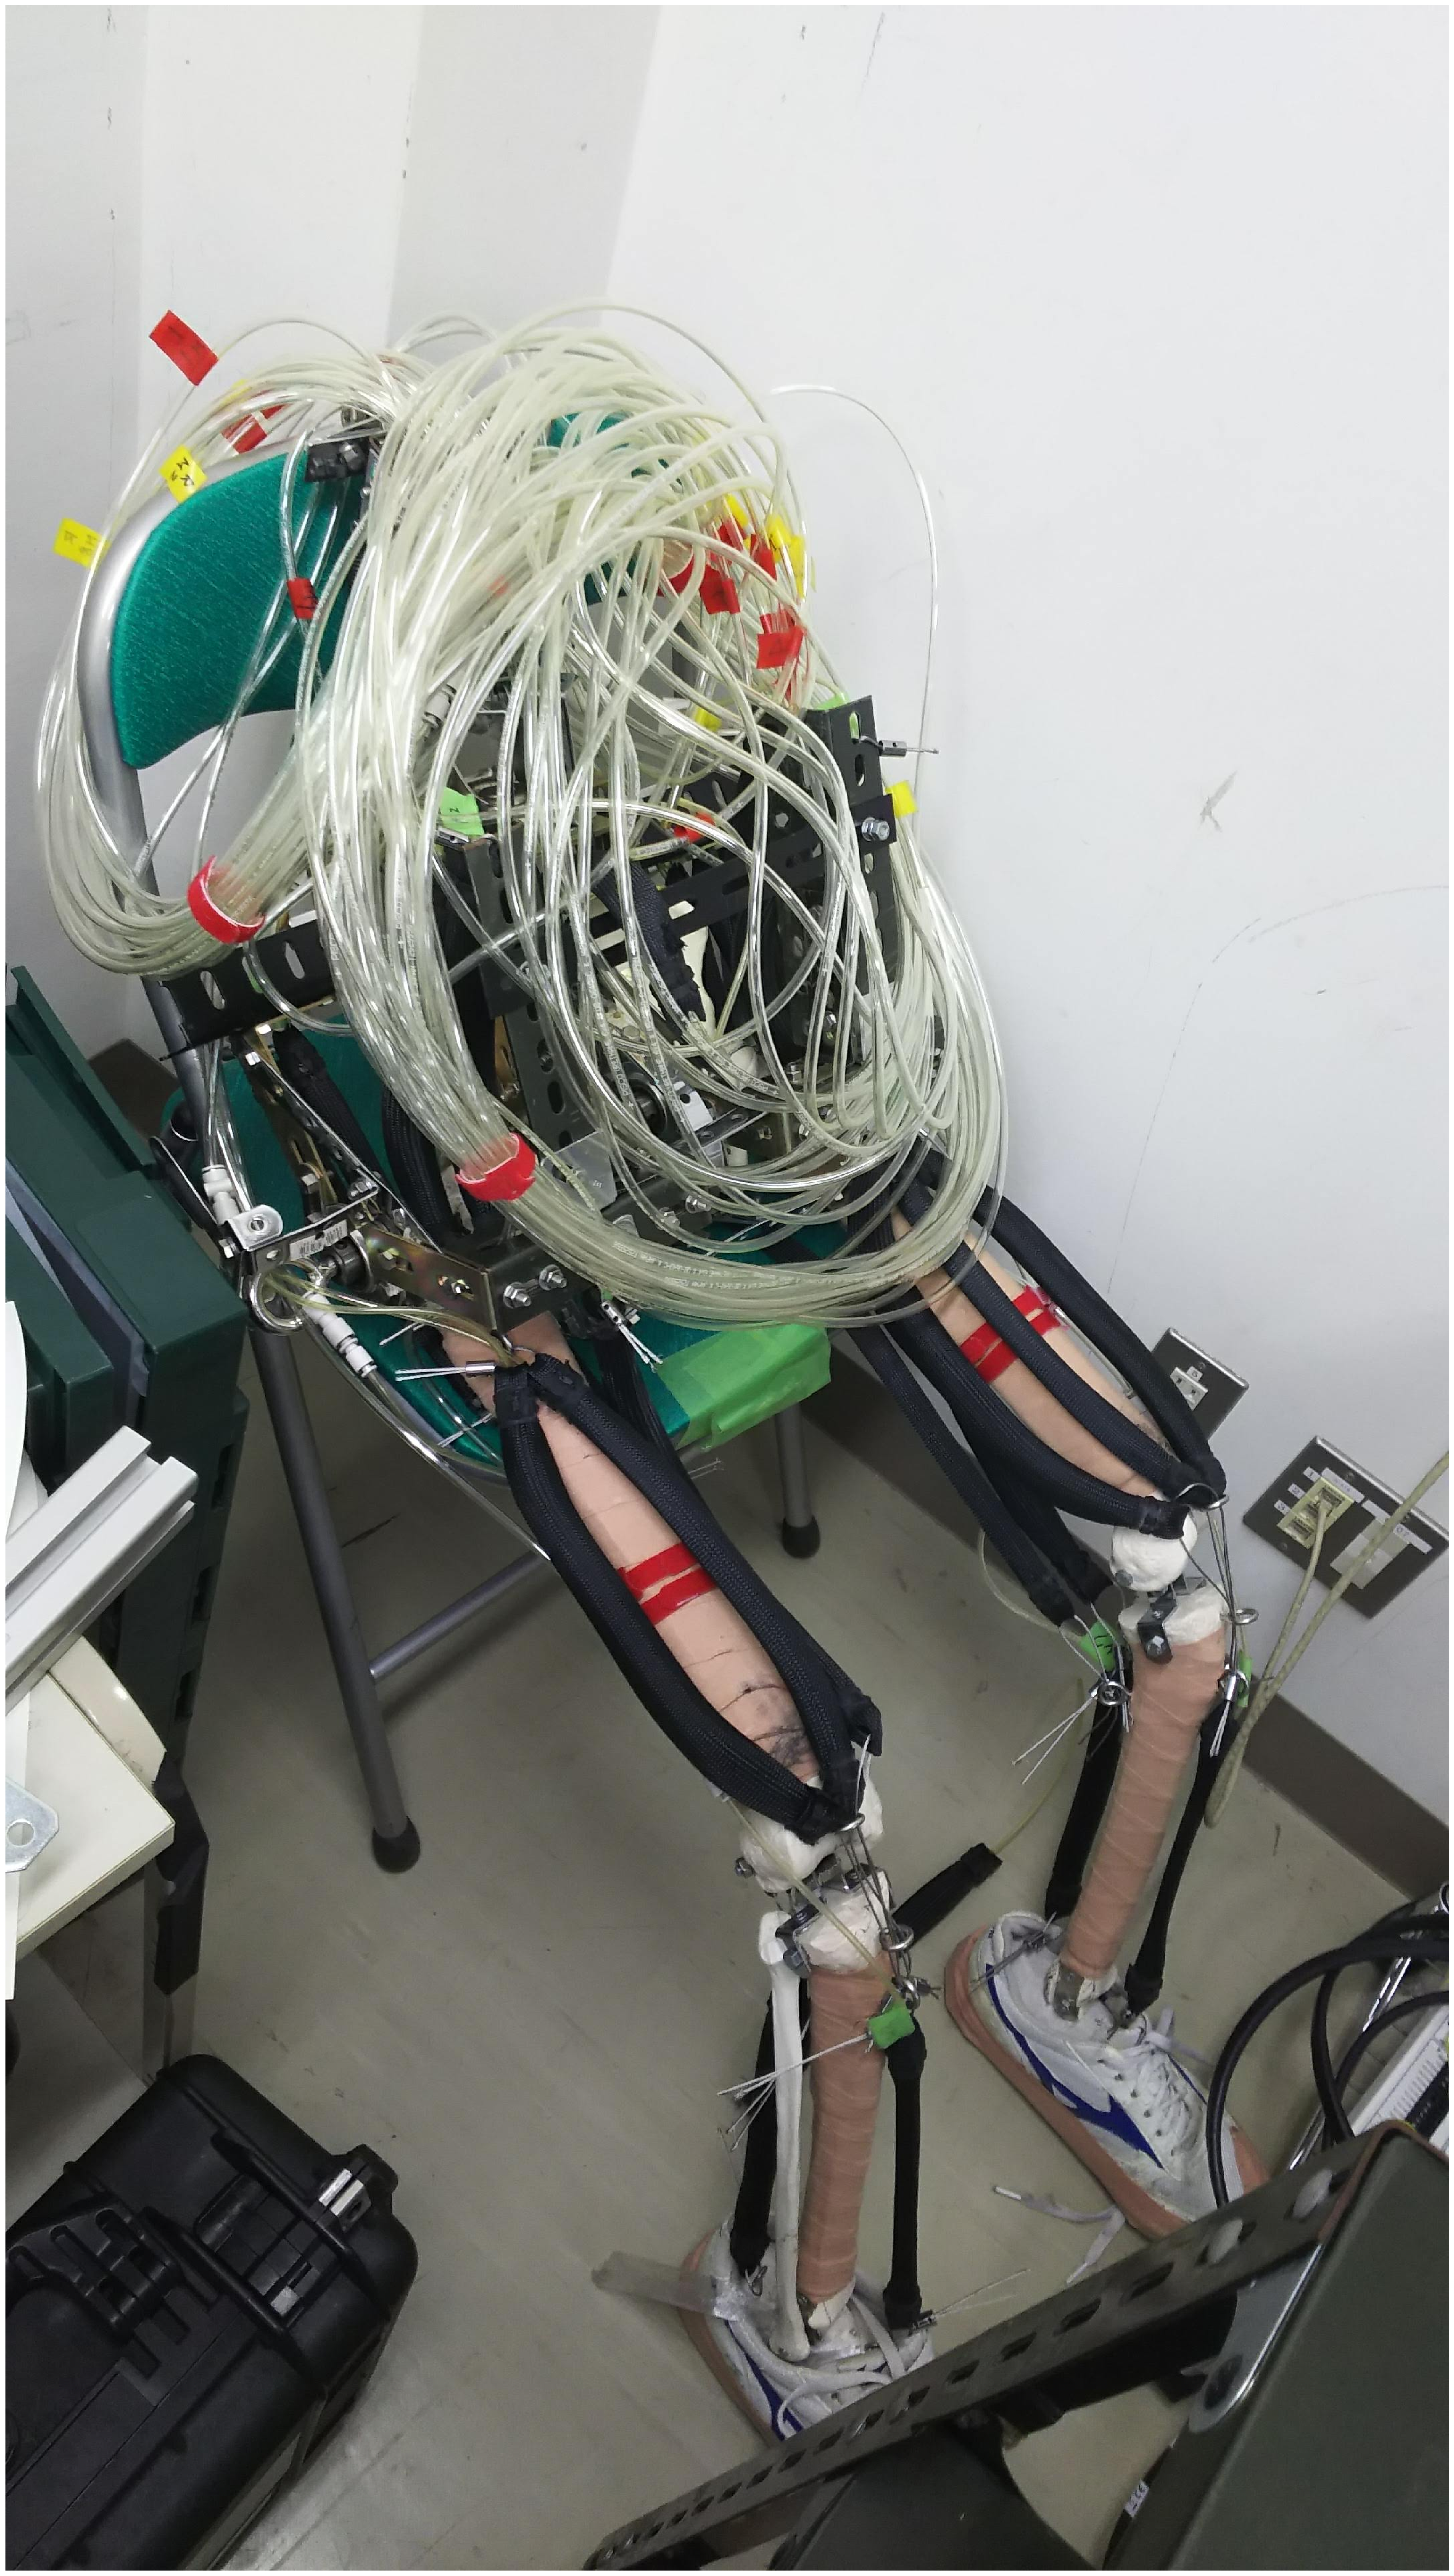
\includegraphics[width=0.5\columnwidth,clip]{Photo/BackGround/2nd.eps}
  \caption{二足歩行ロボット(2号機)}
  \label{2号機}
 \end{center}
\end{figure}

%TODO:2号機のお話を書く
また、これらの機能を利用し二足歩行型のロボットも製作された。こちらは先述のロボットと異なり二足歩行可能であり、片麻痺患者と健常者の歩行の比較を行った。

%TODO:3号機のお話を書く
これら、ペダリングロボット(初号機),2足歩行ロボット(2号機)の経験を踏まえ、今回新たに2足歩行ロボット(3号機)の開発を行った。従来の2足歩行ロボットでは自由度の制約が大きく,2次元平面上のみでの動作となっていたものが3次元空間上で動かせるものとした。

股関節部分の自由度を

足関節の自由度を増加

%TODO:伸縮センサのお話を書く
導電性布を用いて柔軟精度の高いセンサを作成する
空気圧人工筋に本センサーを取り付け
また,これらを利用することで,人間の足首に模した空気圧人工筋をもちいたシステムを動作させる.

%TODO:これらを統合し、筋肉の伸長を巻き込んだシステムの話をする
今回開発を行った導電性布,シリコンを用いた伸縮センサを空気圧人工筋に組み合わせ
\section{動作モデル}
\subsection{足首}
%TODO:足首周りの動作関係のお話をする
%付着筋肉のお話もする
付着筋肉

ボールジョイントを用いて

ロール・ピッチ・ヨー各軸に自由度を持たせた
\subsection{伸縮センサ}
\ref{MITSoftRobot}伸縮センサは
シリコン中に導電性布が2枚挟まれた状態となっている.

これは,誘電体をシリコン,極板を導電性布にしたものとなっている.

ここで伸縮センサ中の導電性布の表面積$S$,誘電体の厚さを$d$とすると、
\begin{eqnarray}
    Q=CV
\end{eqnarray}

比誘電率$\epsilon$とすると

\subsection{伸縮センサ計測回路}
%TODO:伸縮センサ計測回路に関しての記述を行う
\section{実験方法}
\subsection{伸縮センサ作製}
\begin{enumerate}
    \item 3Dプリンターを用いて伸縮センサのサイズに合った型を用意する。
    \item 導電性布を型に合わせて鋏を用いて切る。
    \item 導電性布に錫めっき線を縫い通し、型の上に導電性布を置く.この際、錫めっき線が型の外に出てくるようにする。
    \item 上から硬化剤を混ぜたシリコン流し込み固まるまで数時間放置.
    \item シリコンが固まったら2枚目の導電性布に1枚目と同様に錫めっき線を通し硬化したシリコンの上に置く。
    \item その上から硬化剤を混ぜたシリコンを薄く塗り固まるまで放置.
    \item 最後のシリコンが硬化したら型から取り外し、錫めっき線に銅線接続し、コネクタをつけて完成.
\end{enumerate}
\subsection{伸縮センサ計測}

\subsection{データ処理}

\section{結果}

\section{考察}

\section{結言}

\small
\begin{thebibliography}{99}
%%%%%%%%%%%%%%%%%%%%%%%%%%%%%%%%%%%%%%%%%%%%%%%%%%%%%%%%%%%%%%%%%%%%%%%%%%%%%%%
\bibitem{MITSoftRobot} https://softroboticstoolkit.com/resources-for-educators/tsh-sensor
%%%%%%%%%%%%%%%%%%%%%%%%%%%%%%%%%%%%%%%%%%%%%%%%%%%%%%%%%%%%%%%%%%%%%%%%%%%%%%%
\end{thebibliography}
\normalsize
